%! Author = jonathan
%! Date = 5/27/25
\chapter{Programming Abstractions}\label{ch:abstraction}
\section{Task}\label{sec:task}
We describe the FFN in \S\ref{sec:comoutational-cost-equivalence}, so here we explicate the \emph{combine} operation.
The expert-combine operation, used in architectures like GShard~\cite{DBLP:conf/iclr/LepikhinLXCFHKS21}
and DeepSeek~\cite{deepep}, merges outputs from multiple experts by computing a weighted combination based
on their affinity scores:
\begin{equation}\label{eq:combine1}
\mathcal{C}_i = \sum\limits_{j = 1}^k g_{i, e}
\end{equation}
\begin{equation}\label{eq:combine2}
\mathbf{h}_i = \sum\limits_{j = 1}^k \frac{g_{i, e}}{\mathcal{C}_i}\cdot \mathbf{h}_i^k
\end{equation}
Above, $i \in {0, S - 1}$ represents an input token index, $e = E_{i,k}$ identifies the $k$-th expert
selected for token $i$, and $g_{i,e}$ is the affinity score indicating how relevant expert $e$ is for token $i$.
\section{Unified Abstraction}\label{sec:unified-abstraction}
We unify the FFN and combine operations under a common abstraction called a \emph{task}.
Tasks provide a uniform interface for communicating tile-level work among Subscribers, Schedulers, and Processors.
Formally, a task descriptor $t \in \mathcal{T}$ is defined as a tuple:
\[
    t = (\mathcal{M}, \star, \phi)
\]
where $\mathcal{M}$ is a set of metadata (such as device ID, tile index), $\star$ is a binary tensor operation
(specifically, matrix multiplication $\cdot$ or Hadamard product $\odot$), and $\phi$ is an element-wise activation
function (e.g., ReLU or identity).
We define a task $t$ operating on input tensors $A$, $B$, $D$, producing output tensor $C$, as follows:
\begin{equation}\label{eq:task_def}
\mathcal{F}_t(A, B, C, D) \coloneqq C \gets \phi\left(A \star_t B + D\right)
\end{equation}

The operator $\star_t$ (instantiated from $\star$) may behave differently depending on the task metadata $\mathcal{M}$,
and the result of $A \star_t B$ is accumulated into $D$.
We provide an example of task metadata in Figure \ref{fig:task}.
\begin{figure}[!ht]
    \centering
    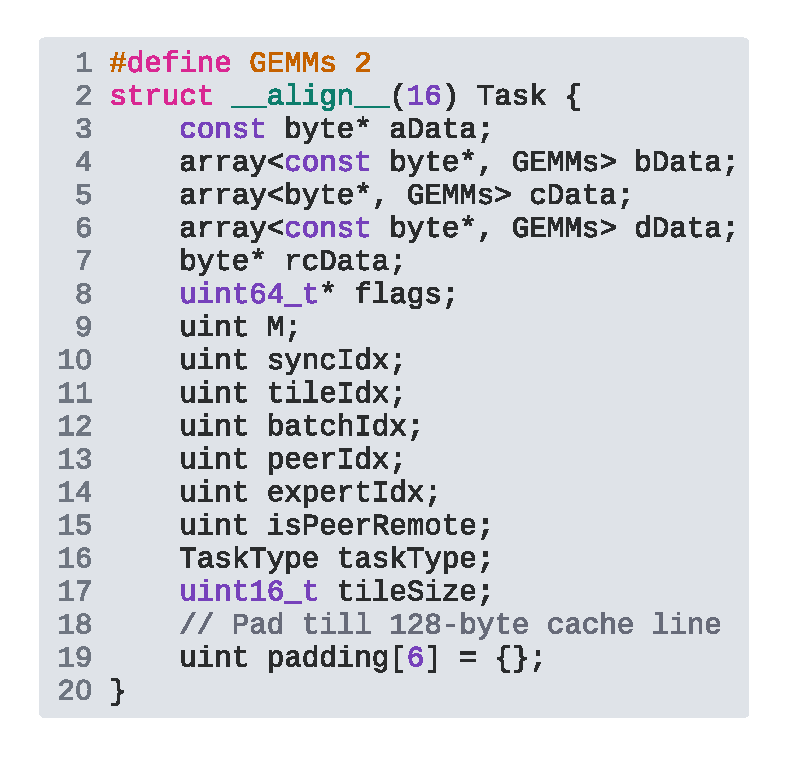
\includegraphics[width=4in]{figures/task}
    \caption{\emph{Task Struct}. $\text{TaskType} \in \{GEMM_0,\>GEMM_1,\>Combine\}$}
    \label{fig:task}
\end{figure}

In practice, we implement each task defined by Equation~\ref{eq:task_def} as a \emph{single fused} \verb|__device__|
decorated function which the \textbf{Processor} (Algorithm \ref{alg:processor}) invokes at runtime.
Fusion for $t$ entails applying $\phi$ and the succeeding addition operation to registers
storing the results of the binary operator $\star_t$.
To illustrate its flexibility, we show how the FFN and expert-combine operations can be expressed
using this task framework.
Note that we omit the matrix multiplication symbol ($\cdot$) for simplicity.
Also, $\phi_1$ can be any activation function, while $\phi_2$ is the identity function.
The FFN is expressed as:
\begin{gather*}
    t_1 = (\mathcal{M}, \cdot, \phi_1), \quad t_2 = (\mathcal{M}, \cdot, \phi_2), \\
    \mathcal{F}_{t_1}(A, B_1, C_1, D_1) \coloneqq C_1 \gets \phi_1\left(A B_1 + D_1\right), \\
    \mathcal{F}_{t_2}(C_1, B_2, C_2, D_2) \coloneqq C_2 \gets \phi_2\left(C_1 B_2 + D_2\right).
\end{gather*}
Whereas, the expert-combine operation is formalized as:
\begin{gather*}
    t_3 = (\mathcal{M}, \odot, \phi_2), \\
    \mathcal{F}_{t_3}(A, S, C, C) \coloneqq C \gets \phi_2\left(A \odot S + C\right).
\end{gather*}
\section{Symmetric Tensor Layout for Inter-GPU Communication}\label{sec:symmetric-tensor-layout}
\begin{figure}[!ht]
    \centering
    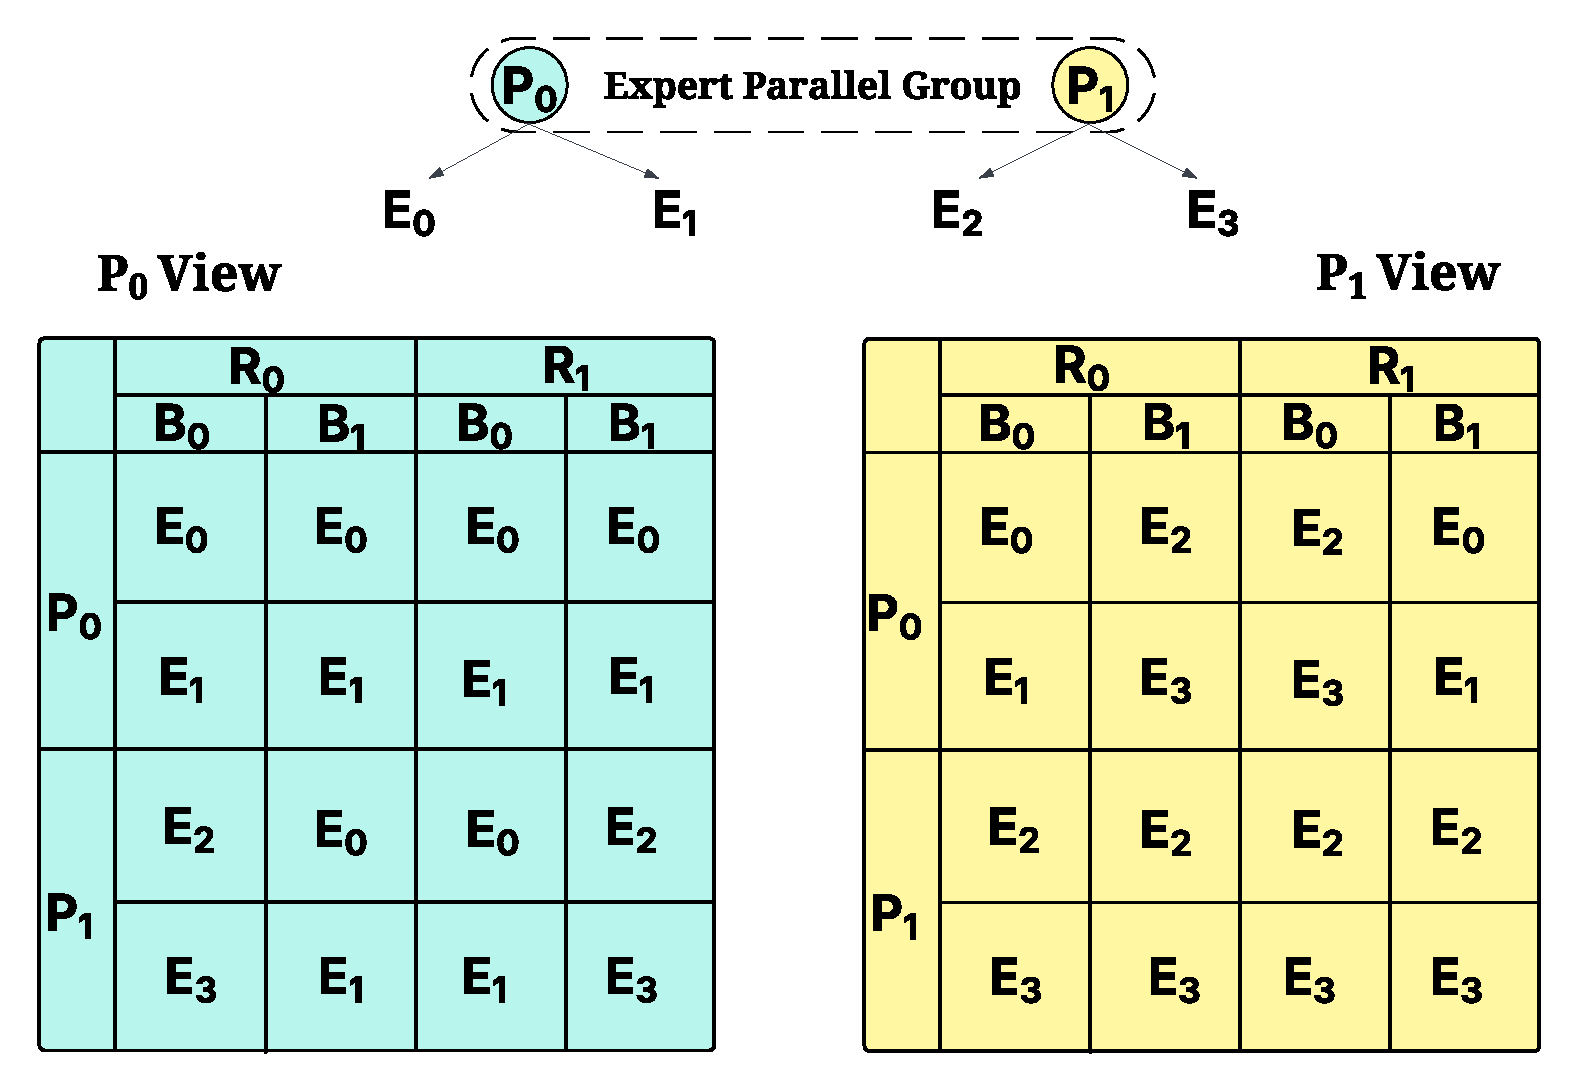
\includegraphics[width=0.85\linewidth, keepaspectratio]{figures/mem_layout}
    \caption{\emph{Symmetric Tensor Layout across 2 Expert-parallel Processes}.}
    \label{fig:mem_layout}
\end{figure}
Within a single GPU device, the actors in \sysname communicate through the GPU's memory subsystem (see Figure~\ref{fig:mem}).
Specifically, the Scheduler and Subscriber actors exchange data via fast shared memory, while other actor
pairs communicate through global memory.
For communication across multiple devices, \sysname uses \emph{device-initiated communication},
leveraging the one-sided PGAS (Partitioned Global Address Space) programming model~\cite{10.1145/1278177.1278183}.
However, achieving scalable and correct one-sided memory accesses in PGAS without costly synchronization
is a known challenge~\cite{deepep, triton-dist}.
We address this challenge with a provably correct and scalable solution: a symmetric tensor layout $L$,
supporting fully non-blocking memory accesses.
We define L as:\\
\[
    L \in \mathbb{R}^{P\times R \times B \times E \times C \times H}
\]
where: $P$ is the expert parallel world size, $R$ identifies communication rounds
(two rounds, one for token dispatch and one for combine), $B$ is number of staging buffers,
$E$ is the number of local experts, $C$ is the upscaled expert capacity (\S\ref{sec:payload})
and $H$ is the embedding dimension.
\begin{figure}[!ht]
    \centering
    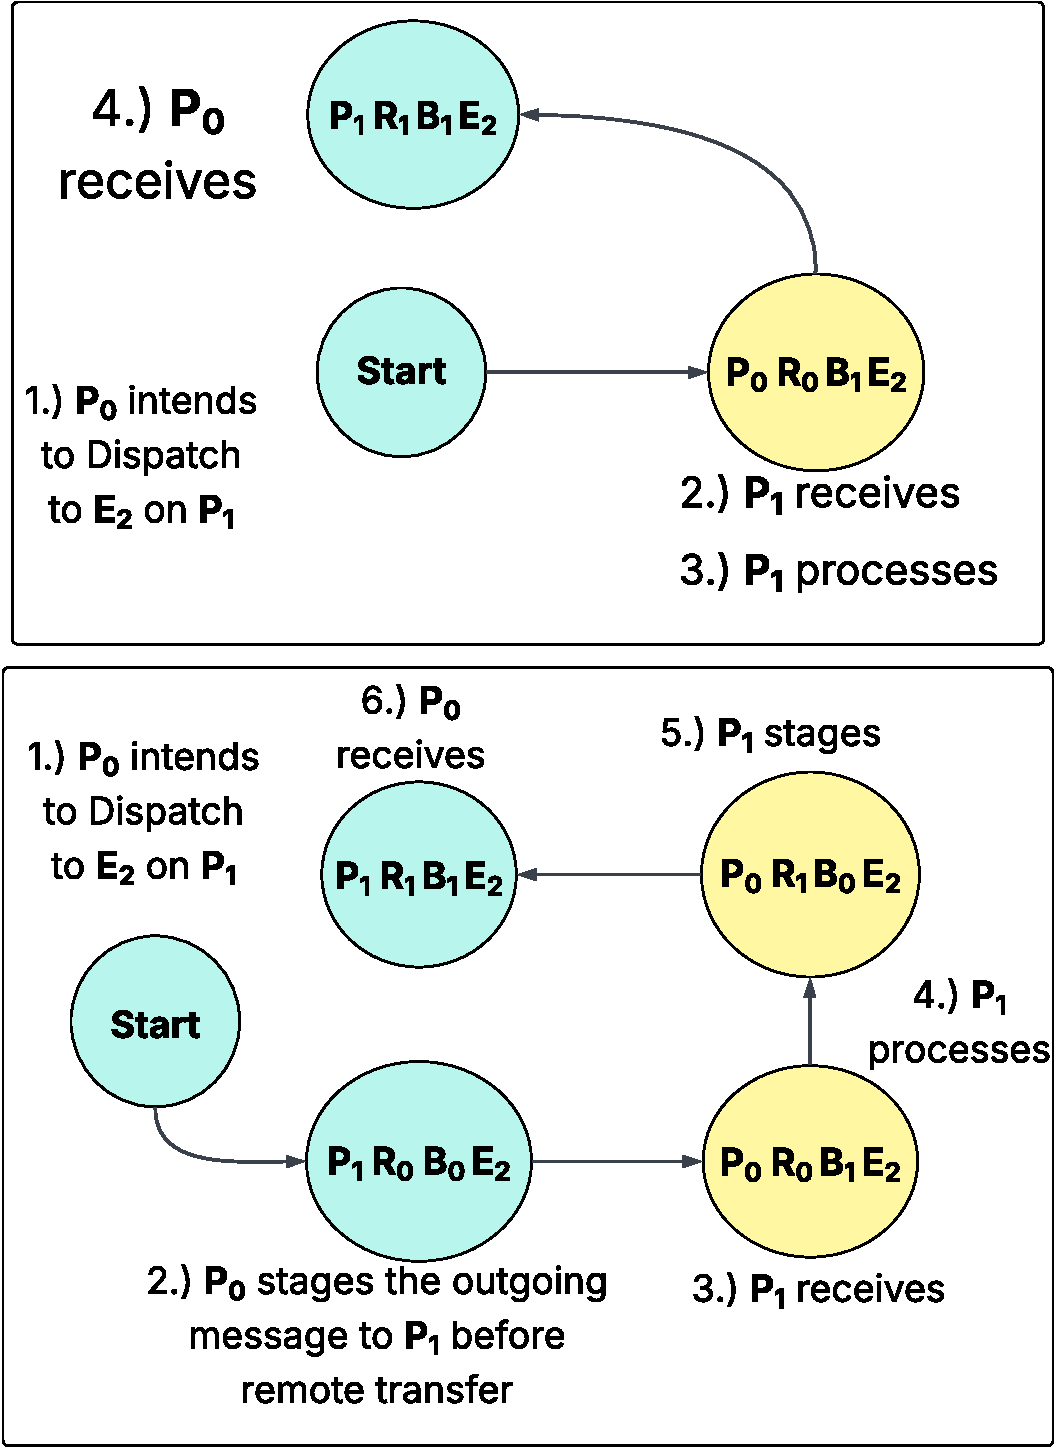
\includegraphics[width=0.7\textwidth, keepaspectratio]{figures/sm_big}
    \caption{\emph{State machine for DMA (top) and RDMA (bottom) communication.}}
    \label{fig:sm}
\end{figure}
Our core insight to enable non-blocking communication is \emph{temporal buffering}.
Specifically, we overprovision memory for the underlying token matrix by at least $2 \cdot r$ times, where $r$ is the number of communication rounds in the dependency graph, and the factor of $2$ accounts for separate buffers for incoming and outgoing data within each communication round. For MoE models, we have $2 \cdot r = 4$.
This modest increase in memory usage eliminates the need for synchronization during one-sided data transfers.
Figure~\ref{fig:sm} illustrates how cells within this symmetric tensor layout are indexed
and used for Direct Memory Access (DMA) and Remote DMA (RDMA) operations.
As Theorem~\ref{theorem:ww} reinforces,
this indexing scheme over $L$ is the underlying mechanism that allows for fully non-blocking accesses eliding
synchronization because all accesses are write \emph{conflict-free}.
\begin{definition}
    Define a write as~$w(p_s, p_t, i)$, where $p_s$ is the source process and $i$ is an ordered tuple
    indicating the index coordinates for $L$ residing on the target process $p_t$.
    A write-write conflict occurs when there exist at least two distinct, un-synchronized, concurrent writes
    $w_1(p_{s_1}, p_{t_1}, i_1)$ and $w_2(p_{s_2}, p_{t_2}, i_2)$, such that
    $p_{t_1} = p_{t_2}$ and index coordinates $i_1 = i_2$ but $p_{s_1} \neq p_{s_2}$
\end{definition}
\begin{definition}
    For any source process $p_s$, a valid index coordinate $i = (p*, r, b, e, c)$ satisfies the following:
    \begin{enumerate}
        \item For inter-device writes, it must hold that $p* = p_s$ and $b = 1$.
        Note this also applies to self-looping writes $w(p_t, p_t, i)$.
        \item For any write $w(p_s, p_t, i)$, if $b = 0$, then $p_s = p_t$.
        This rule describes intra-device staging writes.
    \end{enumerate}
\end{definition}
\begin{theorem}\label{theorem:ww}
$L$ is write-write conflict-free.
\end{theorem}
\begin{proof}
    As is the case for typical physical implementations,
    assume that each index coordinate $i$ maps to a distinct memory segment in $L$.
    Next, we show by contradiction that no write-write conflicts can exist when accessing $L$ using \emph{valid} $i$.
    For simplicity, we only include the index coordinates when describing a write.
    Assume that there exist at least two writes $w_1(p_{s_1}, p_{t_1}, i_1),\>w_2(p_{s_2}, p_{t_2}, i_2)$
    with $p_{t_1} = p_{t_2}$ and valid destination coordinates
    $i_1, i_2$, where $i_1 = i_2$ lexicographically and both are unpacked below.
    \[
        i_1 = (p_1, r_1, b_1, e_1, c_1),\> i_1 = (p_2, r_2, b_2, e_2, c_2)
    \]
    Note that for the message staging state, even though $i_1 = i_2$ the resultant memory segments reside in
    different physical buffers resident in $p_{s_1}$ and $p_{s_2}$ respectively.
    Therefore, for this state, there are no conflicts as intra-process writes always have distinct $c_j$
    coordinates, where $j \in \{0, C - 1\}$.
    For inter-process transfers, we have two cases.

    \textit{Case 1: $p_{s_1} = p_{s_2}$}
    \newline Here, $w_1$ and $w_2$ are identical operations.
    This contradicts the definition of a conflict, which requires that $p_{s_1} \neq p_{s_2}$.
    In practice, such repeat writes never even occur.

    \textit{Case 2: $p_{s_1} \neq p_{s_2}$}
    \newline To ensure validity for $i_1$ and $i_2$, it is the case that $p_1 = p_{s_1}$ and $p_2 = p_{s_2}$.
    However, this implies that $i_1 \neq i_2$ yielding a contradiction as desired.
\end{proof}
To construct $L$, we start from the original token buffer $T \in \mathbb{R}^{S \times H}$, where $S$ is the sequence length and $H$ is the hidden dimension. We first reorganize the sequence dimension $S$ into three sub-dimensions representing the expert capacity ($C$), local expert slots ($E$), and the expert parallel world size ($W$), st:
\[
    C \cdot E \cdot W = C \cdot E' = S', \quad\text{where}\quad S' \geq S \text{ and } E' \geq E_W
\]
In the typical case of uniform expert distribution (illustrated in Figure~\ref{fig:mem_layout}),
we have $S' = S$ and $E' = E_W$, where $E_W$ is the total number of experts in the model.
Thus, the size of the token buffer is $Size(T) = S' \cdot H$.
In Figure~\ref{fig:mem_layout}, each cell labeled $E_i$ (with $i \in \{0,\ldots,3\}$) is a matrix of size $(C, H)$.
Extending prior work~\cite{DBLP:conf/iclr/LepikhinLXCFHKS21, comet}, we introduce additional temporal dimensions $R$
(communication rounds) and $B$ (staging buffers).
Each communication round has two fixed staging slots:
one for outgoing tokens and another for incoming tokens.
Each slot, indexed by dimension $P$, forms a tensor of shape $(S', H)$.
Therefore, the tensor size $Size(L)$ is generally at least four times the original token buffer size,
becoming exactly four times larger in the case of uniform expert distribution.
Empirically (\S\ref{sec:eval:memory}), we find:
\[
    Size(L) \approx 4 \cdot Size(T)
\]
\section{In-place Padding for Payload Efficiency}\label{sec:payload}
Due to the dynamic and uneven distribution of tokens in MoE dispatch~\cite{bmamba},
GPUs commonly receive fewer tokens than their predefined expert capacity.
Current MoE frameworks~\cite{pmlr-v162-rajbhandari22a}
typically pad these buffers with null tokens before computation,
unnecessarily increasing communication payloads and degrading performance.
In contrast, we propose \emph{in-place padding},
performing padding directly within the local symmetric tensor buffers and
thus eliminating excess network communication.
As we show in Figure~\ref{fig:mem_layout} as a reference,
each cell $E_i$ is sized according to the expert capacity $C$.
We further align this capacity to ensure divisibility by the tile block size $bM = 128$,
guaranteeing safe and aligned memory reads by Processor threads consuming remote tokens.
This in-place padding strategy slightly increases the memory footprint of $L$, as described below:
\[
    Size(L) \approx \begin{cases}
                        4 \cdot Size(T), & \frac{S}{E} \geq bM \\[1ex]
                        4 \cdot \frac{bM \cdot E}{S} \cdot Size(T), & \text{otherwise}
    \end{cases}
\]